\section{Integrable chiral gapless phase}
\subsection{Magnetization of Heisenberg chain}
\begin{frame}{Magnetization of Heisenberg chain}
\begin{block}{}
    \begin{equation*}
    \begin{aligned}
        H(J, \alpha) =
        J \sum_{n} \mathbf{s}_n \mathbf{s}_{n+1}
        - h \sum_{n} \mathbf{s}_n.
    \end{aligned}
    \end{equation*}
\end{block}

\begin{block}{Magnetization}
    \begin{columns}[t]
        \column{0.32\textwidth}
        \centering
        \fbox{\parbox{0.75\linewidth}{\centering external field}}
        $\implies$
        \column{0.32\textwidth}
        \centering
        \fbox{\parbox{0.75\linewidth}{\centering $SU(2)$ symmetry breaking}}
        $\implies$
        \column{0.32\textwidth}
        \centering
        \fbox{\parbox{0.9\linewidth}{\centering Magnetization accumulates with any non-zero external field}}
    \end{columns}

Around the critical point:
\begin{equation*}
    m \sim
    \begin{cases}
        \frac12 - \frac{1}{\pi}\sqrt{h_c-h}, h<h_c \\
        \frac12, h>h_c
    \end{cases}
\end{equation*}
\end{block}

\end{frame}
%----------------------------------------------------------------------------------------
\subsection{Heisenberg chain with chiral interaction}
\begin{frame}{Heisenberg chain with chiral interaction}
\begin{equation*}
    H(J, \alpha) =
    \eqnmarkbox[NavyBlue]{HJ}{J \sum_{n} \mathbf{s}_n \mathbf{s}_{n+1}}
    + \eqnmarkbox[WildStrawberry]{Halpha}{\alpha \sum_{n} \mathbf{s}_n \cdot (\mathbf{s}_{n+1} \cross \mathbf{s}_{n+2})}.
\end{equation*}
\annotate[yshift=-0.5em]{below,left}{HJ}{$H_J$}
\annotate[yshift=-0.5em]{below, right}{Halpha}{$H_{\alpha}$}

\vspace{0.5cm}

\begin{block}{Integrablity}
\begin{itemize}
    \item $H_J = \frac{iJ}{2}\left.\frac{\mathrm{d}}{\mathrm{d}u}\ln T(u)\right|_{u=i/2}-\frac{JN}{4}$
    \item $H_{\alpha} = \left. -\frac{i}{4} \frac{d^2}{du^2} \ln T(u) \right|_{u=i/2}
     +\frac{1}{4} iN$
    \item $[H_J , H_{\alpha}] = 0$
\end{itemize}
\end{block}

\end{frame}
%----------------------------------------------------------------------------------------
\begin{frame}{Heisenberg chain with chiral interaction}
\begin{equation*}
\begin{aligned}
    H(J, \alpha) =
    J \sum_{n} \mathbf{s}_n \mathbf{s}_{n+1}
    + \alpha \sum_{n} \mathbf{s}_n \cdot (\mathbf{s}_{n+1} \cross \mathbf{s}_{n+2}).
\end{aligned}
\end{equation*}


critial points: $\alpha_c / J = 2 / \pi$

\begin{columns}
    \begin{column}{0.6\textwidth}
        \begin{figure}
            \centering
            \begin{minipage}{0.45\linewidth}
            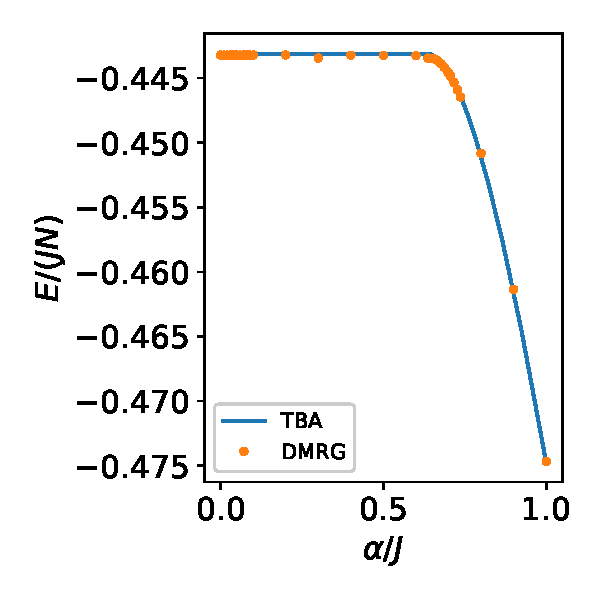
\includegraphics[width=\textwidth]{figs/CSC/Ealpha.pdf}
            \end{minipage}
            % 
            \begin{minipage}{0.45\linewidth}
            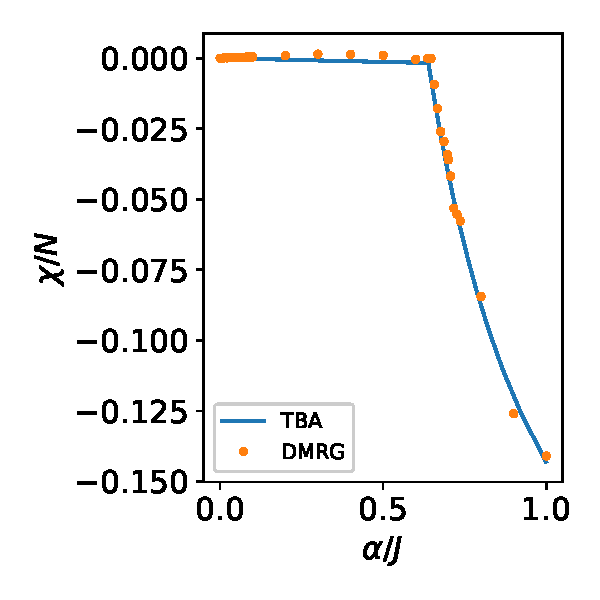
\includegraphics[width=\textwidth]{figs/CSC/chialpha.pdf}
            \end{minipage}
        \end{figure}
    \end{column}
    \begin{column}{0.3\textwidth}
        \begin{equation*}
            \chi \sim
            \begin{cases}
                0, \alpha<\alpha_c \\
                \alpha_c - \alpha, \alpha>\alpha_c
            \end{cases}
        \end{equation*}
        At low temperature and small $\alpha$: 
        % \begin{equation*}
            $\chi \sim -\alpha T^2$
        % \end{equation*}
    \end{column}
\end{columns}
\end{frame}
%----------------------------------------------------------------------------------------
\subsection{Symmetry-enriched CFT}
\begin{frame}{Symmetry-enriched CFT}

\begin{block}{Heisenberg criticality}
    When $\alpha < \alpha_c$, the phase is in the same universality class of the Heisenberg criticality.
    The primary field is associated with spin flip $s_x$
    \begin{equation*}
    (\mathcal{PT})^{-1} s^x \mathcal{PT} = -s^x
    \end{equation*}
    where $\mathcal{P}$ is the parity inversion and $\mathcal{T}$ is the time reversal.
\end{block}

\end{frame}
%----------------------------------------------------------------------------------------
\begin{frame}{Symmetry-enriched CFT}

\begin{block}{Chiral Heisenberg criticality}
    When $\alpha > \alpha_c$, the primary field is related to a phase twist $p$
    \begin{equation*}
    (\mathcal{PT})^{-1} p (\mathcal{PT}) = p
    \end{equation*}

    \begin{itemize}
        \item 
        % \begin{equation*}
        $p \equiv \prod_{n=1}^L P_n\left(\frac{2\pi n}{N} - \pi n(N + 1) \right)$
        % \end{equation*}

        \item 
        $P_n(\varphi)$ maps the basis states $\ket{\downarrow} \to \ket{\downarrow}$ and $\ket{\uparrow} \to e^{i\varphi}\ket{\uparrow}$

        % \item $\Pi: \mathbb{Z}\rightarrow\{0,1\}$ is the parity of the argument
    \end{itemize}
\end{block}

\vspace{-0.5cm}
\begin{equation*}
\begin{aligned}
    \ket{g_1} &=
    \sum_n \exp(\frac{2\pi i n}{N}) \ket{\downarrow,\downarrow, ..., \uparrow_{{\rm site~} n}, ..., \downarrow,\downarrow}, 
    \ket{g_2} =
    \sum_n \exp(-\frac{2\pi i n}{N}) \ket{\uparrow,\uparrow, ..., \downarrow_{{\rm site~} n}, ..., \uparrow,\uparrow} \\
    \ket{e_1} &=
    \sum_n (-1)^{\Pi[n(N+1)]} \ket{\downarrow,\downarrow, ..., \uparrow_{{\rm site~} n}, ..., \downarrow,\downarrow}, 
    \ket{e_2} =
    \sum_n (-1)^{\Pi[n(N+1)]} \ket{\uparrow,\uparrow, ..., \downarrow_{{\rm site~} n}, ..., \uparrow,\uparrow}
\end{aligned}
\end{equation*}

\vspace{-0.5cm}
This is known as symmetry-enriched CFTs\footnote[frame]{\cite{verresen2021gapless}}

\end{frame}
%----------------------------------------------------------------------------------------
\subsection{Finite size correction}
%----------------------------------------------------------------------------------------
\begin{frame}{Finite size correction}

\begin{block}{How do we distinguish the two phases?}
    \begin{itemize}
        \item $E_{\rm total} = E_{\rm bulk} + E_{\rm finite}$
        \item Heisenberg part: $E_{\rm Heisenberg} = (\ln 2 - 1/4) N + \frac{\pi^2}{12N}$
        \item Chiral part: $E_{\chi} =  -\frac{\pi ^{7/2}}{64 e \left(\sqrt{\pi }-\sqrt{e} \gamma_0\right)} \Delta \alpha^2 N + \frac{cv}{N} f(\Delta \alpha N)$
    \end{itemize}
    % \begin{equation*}
    %     E = \epsilon N + \frac{cv}{N} (f((\alpha-\alpha_c) N) - \frac{\pi}{6})
    % \end{equation*}
\end{block}


\begin{figure}
    \centering
    \begin{minipage}{0.3\linewidth}
    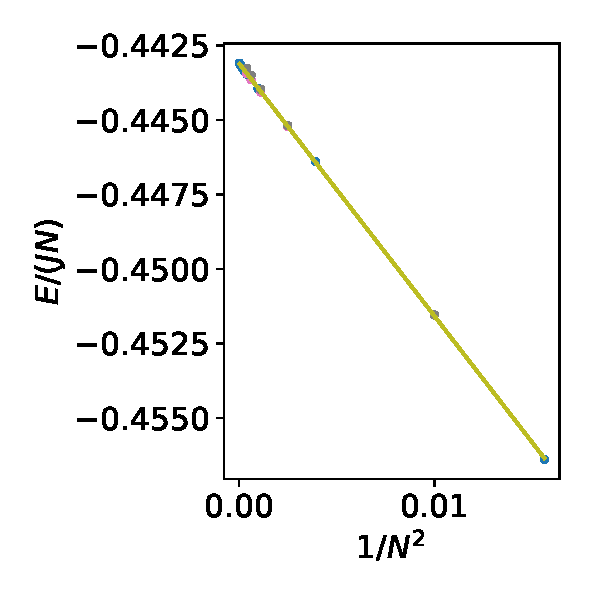
\includegraphics[width=\textwidth]{figs/CSC/E_over_N.pdf}
    \end{minipage}
    %
    \begin{minipage}{0.3\linewidth}
    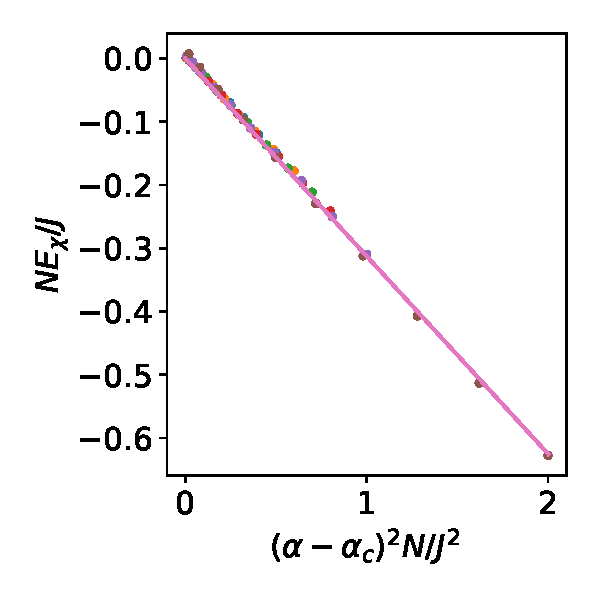
\includegraphics[width=\textwidth]{figs/CSC/E_chi.pdf}
    \end{minipage}
    % 
    \begin{minipage}{0.3\linewidth}
    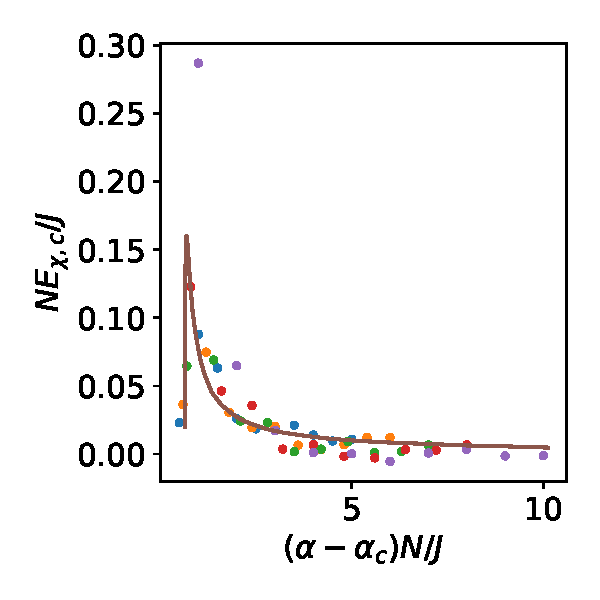
\includegraphics[width=\textwidth]{figs/CSC/E_chi_c.pdf}
    \end{minipage}
%%%%%%%%%%%%%%%%%%%%%%%%%%%%%%%%%%%
\end{figure}
\end{frame}
%----------------------------------------------------------------------------------------
\begin{frame}{Phase diagram}
\begin{columns}
\begin{column}{0.4\textwidth}
    1D spin-1/2 XXZ chain with chiral term

    \begin{equation*}
    \begin{aligned}
        H(J, \Delta, \alpha) =
        &J \sum_{n} s^{(x)}_n s^{(x)}_{n+1}
        + J \sum_{n} s^{(y)}_n s^{(y)}_{n+1} \\
        + &\Delta \sum_{n} s^{(z)}_n s^{(z)}_{n+1} \\
        + &\alpha \sum_{n} \mathbf{s}_n \cdot (\mathbf{s}_{n+1} \cross \mathbf{s}_{n+2})
    \end{aligned}
    \end{equation*}
\end{column}

\begin{column}{0.4\textwidth}
    \begin{minipage}{1.0\linewidth}
    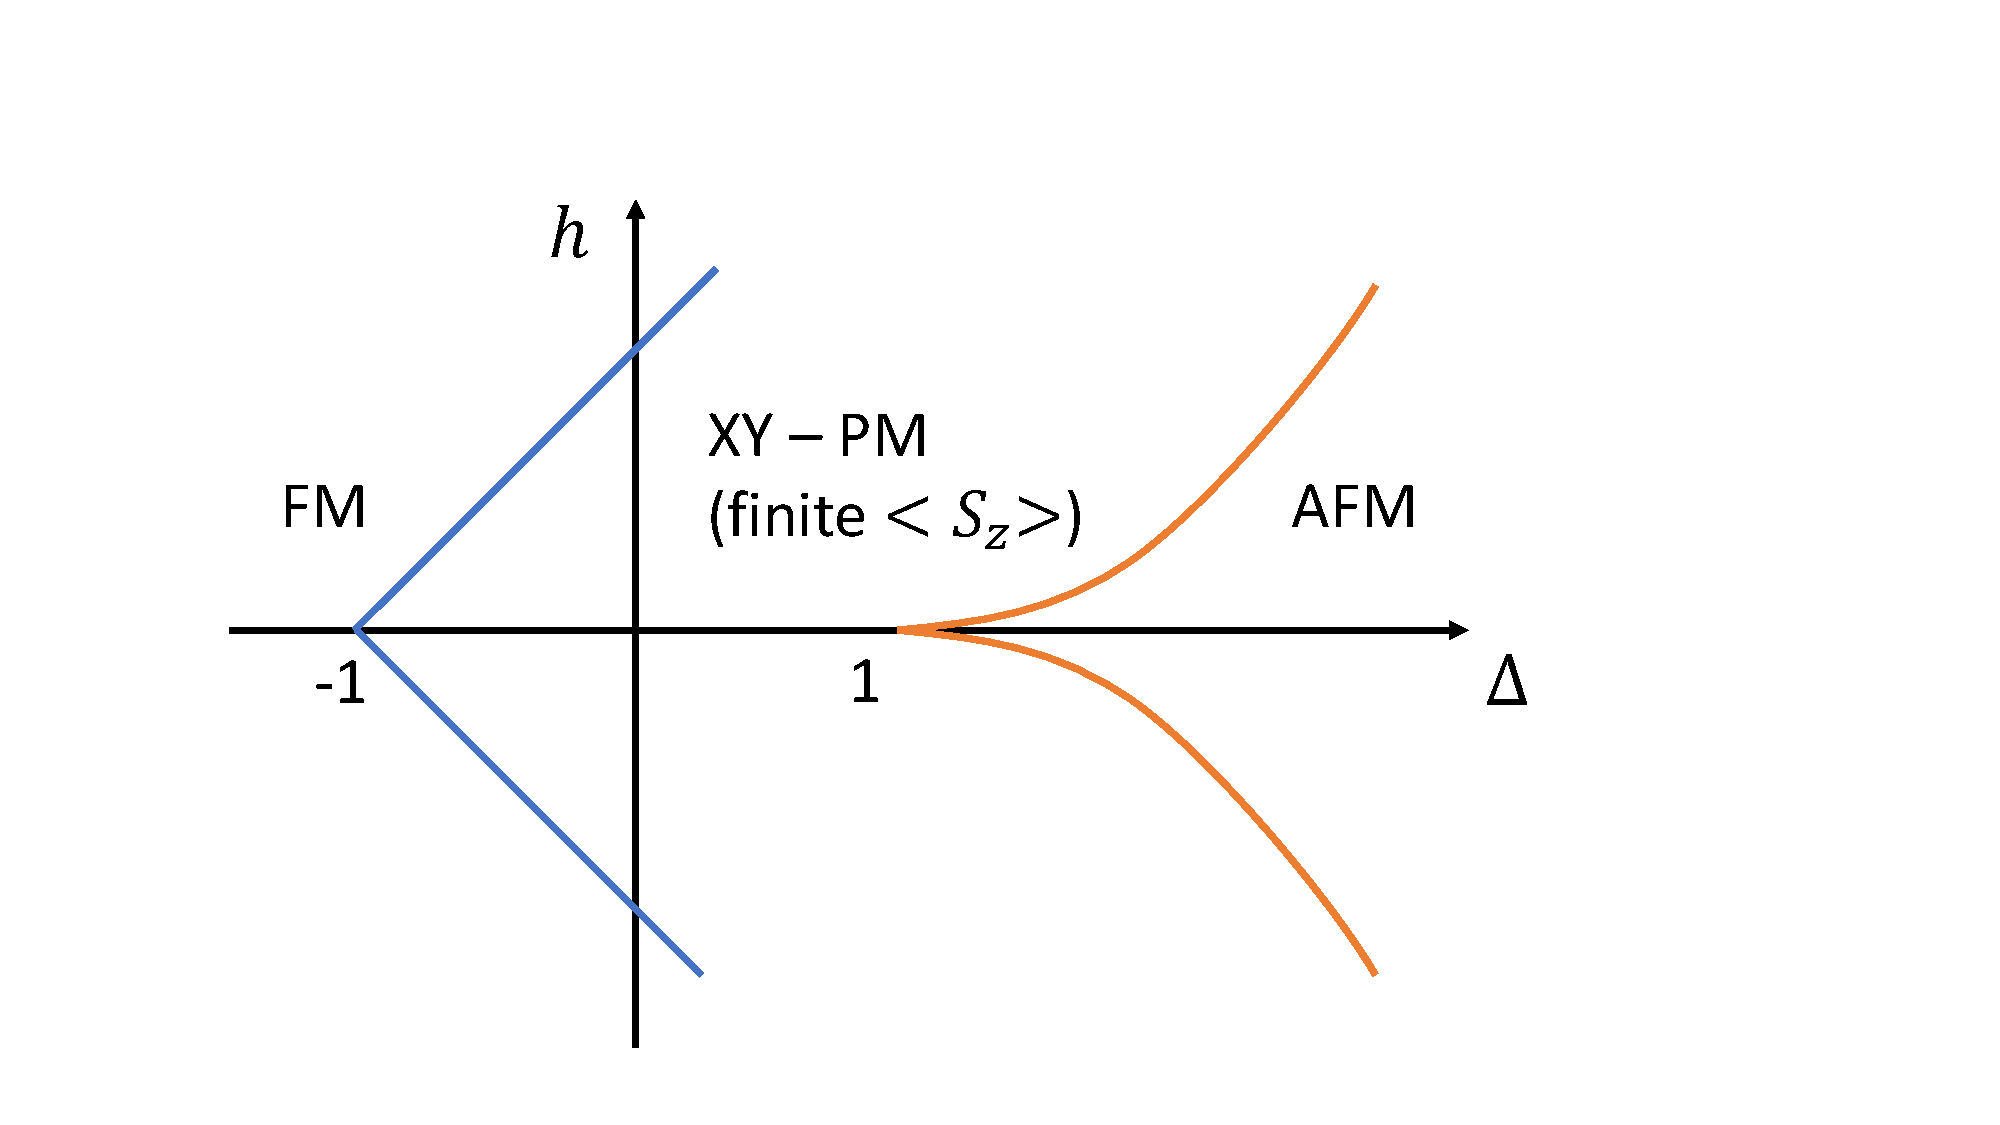
\includegraphics[width=\linewidth]{figs/CSC/phase_diagrams_Heisenberg.pdf}
    \vspace{0.5cm}
    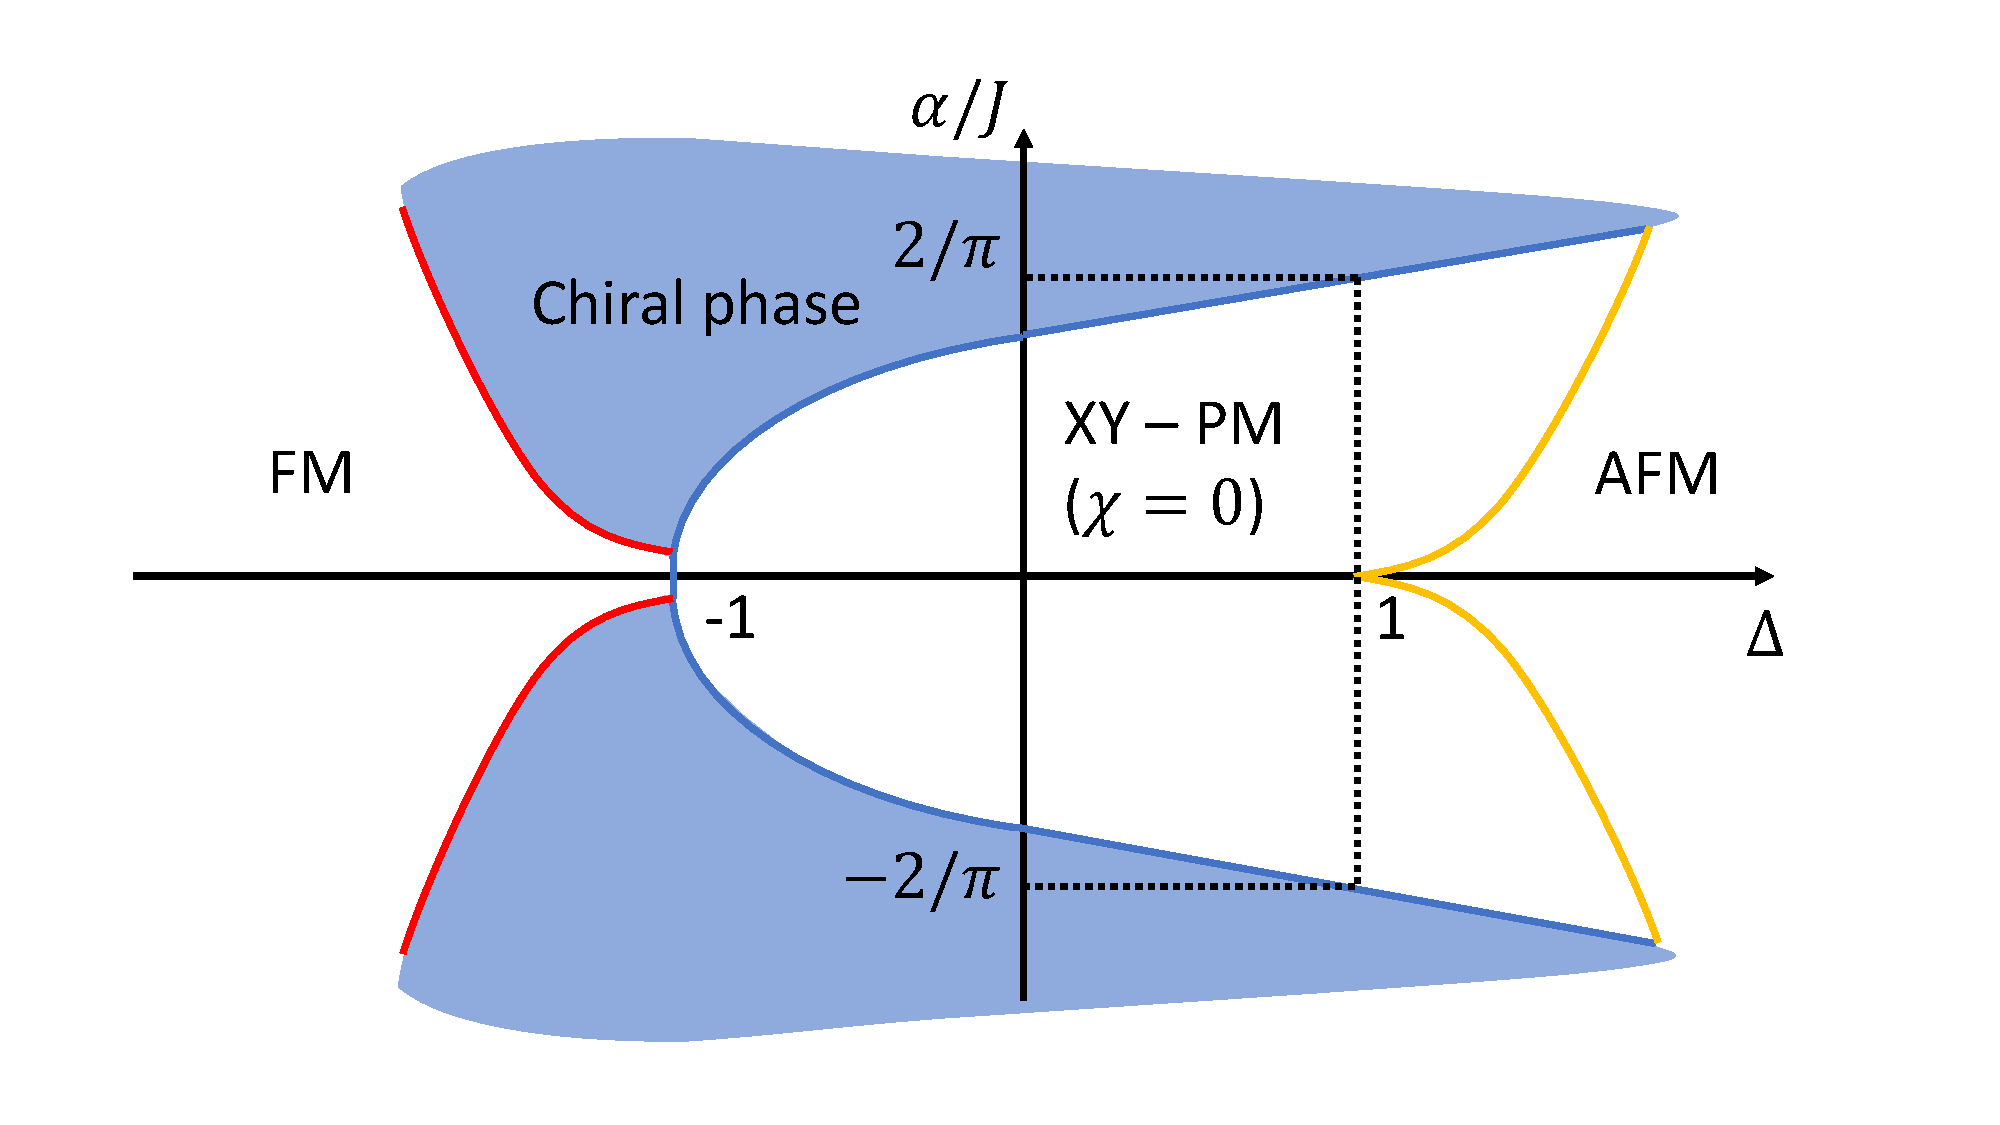
\includegraphics[width=\linewidth]{figs/CSC/phase_diagrams_chiral.pdf}
    \end{minipage}
\end{column}
\end{columns}
\end{frame}
% %----------------------------------------------------------------------------------------
% \subsection{symmetry enriched criticality}
% %----------------------------------------------------------------------------------------
% \begin{frame}{symmetry-enriched criticality}

% \begin{block}{Is there anyway we can tell the difference between the two phases in the thermodynamic limit?}
%     \begin{itemize}
%         \item $ \mathcal{C}^{-1} s_x \mathcal{C} = s_x $
%         \item $ \mathcal{C}^{-1} (\prod s_x) \mathcal{C} = -s_x $
%     \end{itemize}
% \end{block}
% \end{frame}

